\documentclass[border=2pt]{standalone}
\usepackage{pgfplots}
\pgfplotsset{compat=1.18}
\definecolor{red}{rgb}{0.7,0.11,0.11}
\definecolor{blue}{rgb}{0.0,0.20,0.42}
\definecolor{green}{rgb}{0.11,0.35,0.02}
\begin{document}
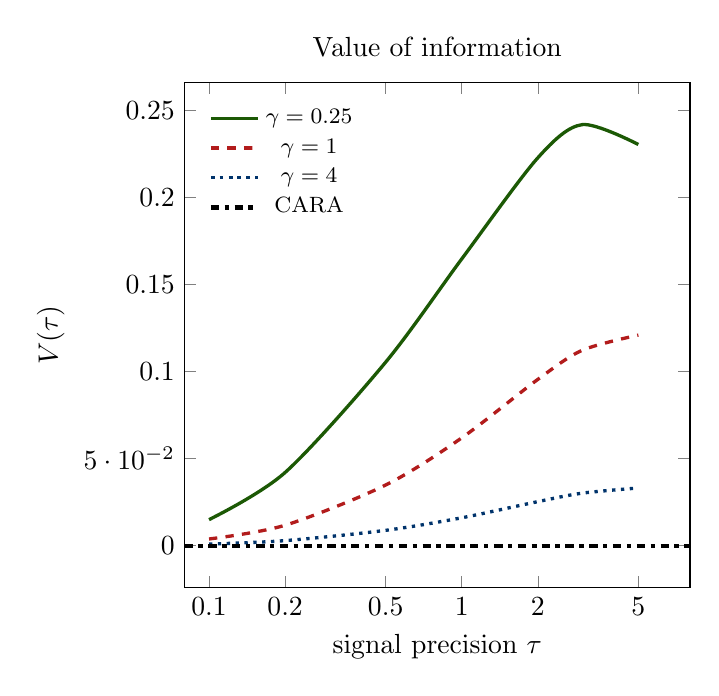
\begin{tikzpicture}
\begin{axis}[
    width=8cm, height=8cm,
    xmode=log,
    xmin=0.08, xmax=8,
    xtick={0.1,0.2,0.5,1,2,5},
    xticklabels={0.1,0.2,0.5,1,2,5},
    xlabel={signal precision $\tau$},
    ylabel={$V(\tau)$},
    title={Value of information},
    legend pos=north west,
    legend style={fill=none, draw=none, font=\footnotesize},
    smooth,
]
\addplot[very thick, color=green, smooth] coordinates {(0.1000,0.0150166) (0.2000,0.0420868) (0.5000,0.10545) (1.0000,0.164733) (2.0000,0.222791) (3.0000,0.241876) (5.0000,0.230454)};
\addplot[very thick, color=red, dashed, smooth] coordinates {(0.1000,0.00389789) (0.2000,0.0117898) (0.5000,0.0348889) (1.0000,0.0619675) (2.0000,0.0955367) (3.0000,0.112293) (5.0000,0.120987)};
\addplot[very thick, color=blue, dotted, smooth] coordinates {(0.1000,0.000977427) (0.2000,0.00295885) (0.5000,0.00886365) (1.0000,0.0160729) (2.0000,0.0253478) (3.0000,0.030226) (5.0000,0.0331742)};
\addplot[ultra thick, color=black, dashdotted]
    coordinates {(0.08,0)(8,0)};
\addlegendentry{$\gamma = 0.25$}
\addlegendentry{$\gamma = 1$}
\addlegendentry{$\gamma = 4$}
\addlegendentry{CARA}
\end{axis}
\end{tikzpicture}
\end{document}
